\chapter{Metodologia}
\label{cha:metodologia}

	O trabalho é executado a partir de revisão bibliográfica de textos acadêmicos, como dissertações e teses, artigos publicados em revistas acadêmicas, livros teóricos e notas de estudos técnicos. A revisão bibliográfica tem o objetivo de se inteirar do estado da arte das tecnologias envolvidas na Indústria 4.0.
	
	As disciplinas obrigatórias do programa de pós-graduação cursadas durante o período do mestrado foram selecionadas com base na relevância e relacionamento com a natureza da pesquisa em Indústria 4.0 e incluem disciplinas também de outros programas de pós-graduação, como o de Engenharia Elétrica, Engenharia de Transportes e Engenharia de Produção.
	
	A metodologia adotada neste projeto será baseada naquela proposta por \citeonline{jensen1997petrinet}, onde as etapas de pesquisa são compostas por um ciclo repetitivo de três aspectos, sendo elas as teorias, ferramentas e aplicações, conforme ilustrado na \autoref{fig:metodologia-jensen}.
	
	O próprio conhecimento adquirido nas disciplinas por meio da aprendizagem de novas “ferramentas” pode modificar parte das “aplicações” e com isso realimentar as “teorias” iniciais. Mediante a evolução do projeto ao longo do tempo, novas propostas surgem, e com isso a necessidade do aprendizado de novos conceitos/teorias.

	\begin{figure}[htb]
		\centering
		\caption{Metodologia de pesquisa utilizada.}
		\label{fig:metodologia-jensen}
		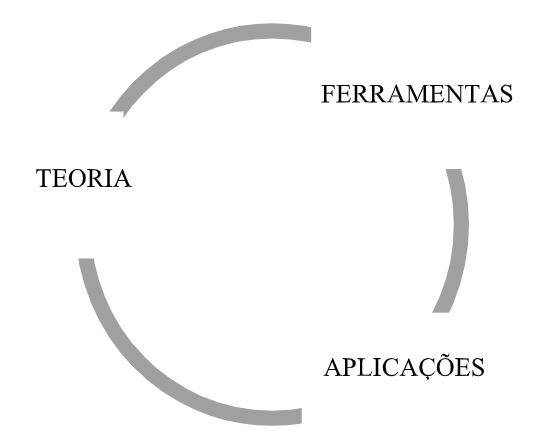
\includegraphics[width=0.7\textwidth]{metodologia-jensen.png}
		\fonte{\citeonline{jensen1997petrinet} (adaptado).}
	\end{figure}


	Aplicando-se a metodologia proposta por \citeonline{jensen1997petrinet} para o caso específico do plano de pesquisa em questão, pode-se listar teorias, ferramentas e aplicações individuais do projeto, formando-se o ciclo mostrado na \autoref{fig:metodologia-jensen}. Os três aspectos identificados na \autoref{fig:metodologia-jensen} devem evoluir simultaneamente, recondicionando-se mutuamente.

